\documentclass[conference]{IEEEtran}

\usepackage{amsmath}
\usepackage{amssymb}
\usepackage{graphicx}
\usepackage{color}
\usepackage[colorlinks,allcolors=blue]{hyperref}

\newcommand{\todo}[1]{\textcolor{red}{/* #1 */}}

\begin{document}
	
	\title{A model for multi-objective optimal multi-modal passenger transport and energy flow control}
	
	\author{
		\IEEEauthorblockN{Dominik Ascher}
		\IEEEauthorblockA{
			Fakult\"at f\"ur Informatik\\
			Technische Universit\"at M\"unchen\\
			85748 Garching bei M\"unchen, Germany\\
			Email: \href{mailto:ascher@in.tum.de}{ascher@in.tum.de}
		}
		\and
		\IEEEauthorblockN{Georg Hackenberg}
		\IEEEauthorblockA{
			Fakult\"at f\"ur Informatik\\
			Technische Universit\"at M\"unchen\\
			85748 Garching bei M\"unchen, Germany\\
			Email: \href{mailto:hackenbe@in.tum.de}{hackenbe@in.tum.de}
		}
		\and
		\IEEEauthorblockN{...}
		\IEEEauthorblockA{
			...
		}
	}

	\maketitle
	
	\begin{abstract}
		\todo{Write abstract.}
	Crucial challenges for future power and transportation systems are imposed by electric vehicles (EV) and renewable energy sources (RES).	
	Increasing integration between transportation and power systems.
	Integrated planing, operation and control strategies for integrated transportation and power systems have to be established.
		
	\end{abstract}
	
	\section{Introduction}
	
	Guaranteeing sustainability and minimizing negative environmental impacts are crucial challenges for future power and transportation systems. Widespread adoption of electric vehicles (EVs) as well as high penetration of renewable energy sources (RES) necessitate substantial changes within these systems. Here, within the power systems, intermittent power outputs require elaborate load balancing strategies while increasing adoption of autonomous electric vehicles requires addressing changing mobility demands in the transportation system. To comprehensively address constraints, objectives and design alternatives of both transportation and power systems, sustainable and integrated planning, operation and control strategies have to be established within integrated transportation and power systems.
	
	According planning, operation and control strategies are frequently addressed within the concept of vehicle-to-grid (V2G). V2G describes a concept, where energy is released from EV batteries to the power system in times of increased power demand.  By facilitating interaction between power system and EVs, V2G possesses the potential to significantly reduce the amount of excess renewable energy produced within the power system \cite{richardson2013electric}. More generally, significant advantages as well as disadvantages can be argued for widespread V2G adoption. Here, both environmental and economic benefits have been shown in the past \cite{faria2012sustainability, richardson2013electric, mwasilu2014electric}. Furthermore, key benefits of V2G include reduction of emissions, increased efficiency as well as stability and reliability of the power system \cite{yilmaz2013review}.
	
	On the contrary, Mwasilu et al.~\cite{mwasilu2014electric} argue that for V2G adoption in a smart grid context central technological issues have to be addressed first such as coping with communication delays, establishing routing protocols and cyber security. Adding to that, the authors argue that frequent charging and discharging cycles causing rapid battery degradation for EV batteries as well as low penetration of electric vehicles with V2G functionality hinder more widespread V2G adoption.
	
	Nevertheless, previous work on plug-in electric vehicles (PEVs) has shown their ability to contribute to balancing the fluctuation of intermittent renewable energy sources \cite{dallinger2012grid}. Currently, V2G represents a supplementary strategy to address situations in the power system with increased power demand. Currently, available intermittent renewable energy sources have to be supplemented with conventional energy sources as well as energy storages within the power system. To achieve a continuous balance between energy supply and demands within power systems, prevalent control schemes rely on automatic control schemes which are supervised by human operators. Here, according control schemes are subject to challenges from increasing levels of fluctuating RES \cite{heussen2012unified}.
	
	Given these current and future challenges and the prospected impact of RES and EVs on such systems, effective integrated control strategies to handle future power and mobility demands still have a long way to go and are subject to ongoing research.
	
	\todo{Sustainability as motivation}
	
	\todo{Multi-objective optimal control?}
	
	\subsubsection*{Outline}
	
	The remainder of the article is structured as follows: Section~\ref{related_work} summarizes related work in the field. Section~\ref{proposed_work} summarizes the contributions of this article. Section~\ref{proposed_model} describes the proposed modeling technique. Section~\ref{discussion} discusses the proposed technique with respect to various quality criteria. Finally, Section~\ref{conclusion} draws a conclusion from our current state of work.
	
	\section{Related work}
	\label{related_work}
	
	In the following we first review related approaches in Section~\ref{approaches} before deriving remaining problems in Section~\ref{problems}.
	
	\subsection{Approaches}
	\label{approaches}
		
	Previous studies have shown that, given a high penetration of EVs, uncontrolled charging can impose increased peak loads within the distribution network \cite{lopes2009identifying}. Intelligent scheduling methods are widely discussed as key approaches to integrate electric vehicles into the power grid \cite{yang2015computational}. According approaches often focus on minimizing single or multiple objectives within given power system models, while restricting valid behavior in terms of a set of constraints. For instance, typical objectives are minimizing cost (or maximizing welfare), power losses, emissions, power deviations or optimizing battery performance of EVs within power systems \cite{yang2015computational}. Here, the power systems are consisted of a number of electric devices such as conventional or renewable energy sources, energy consumers as well as electric infrastructure.
	
	In this context, Andreotti et al.~\cite{andreotti2012review} compare single-objective optimization methods within a smart grid context under the presence of EVs to evaluate model effectiveness in terms of operational limits and used objective functions. In this context, to sufficiently address technical and economic objectives for PEVs, the authors argue higher suitability of multi-objective optimization methods. 
	
	Zakariazadeh et al.~\cite{zakariazadeh2014multi} propose a multi-objective scheduling method for electric vehicles within a smart distribution network addressing economic and environmental objectives as well as technical constraints. Here, the approach manages to reduce operational costs and emissions, achieving Pareto-optimal solutions.
	
	To achieve optimal charging decisions for EVs, Ota et al.~\cite{ota2012autonomous} propose a decentralized V2G control scheme to address the intermittency of RES energy production using electric vehicles. However, the authors focus on the effects of an according charging control scheme within an isolated power system only.
	
	Here, approaches often restrict the impact of electric vehicles to decisions on charging or discharging their batteries at charging stations. However, in subsequence, individual EV objectives describing routing preferences such as shortest traveling time or energy-efficiency for EVs cannot be sufficiently taken into account. Instead, emphasis is put on the power system side, while the transportation system including traffic participants isn't represented microscopically. 
	
	Another highly relevant direction for efficiently integrating electric vehicles into the power grid and reduce negative impacts is are approaches utilizing Vehicle Routing Problems (VRPs). Methods for vehicle routing typically focus on optimizing route selection for single or multiple traffic participants towards single or multiple objectives and a given set of constraints. Addressing objectives of energy-efficiency in terms of routing problems, Eco-Routing approaches target energy-efficient route selection. In contrast, Eco-Driving approaches target energy-efficient intermediate driving behavior ~\cite{ericsson2006optimizing}.
	
	Felipe et al.~\cite{felipe2014heuristic} propose multiple heuristics for routing electric vehicles which consider different partial recharge strategies and recharge technologies while traveling along routes. However, approaches does not take the effects of recharging within the power system into account for general cost evaluation. 
	
	Integrating both scheduling and routing approaches for EV, Barco et al.~\cite{barco2013optimal} present an approach for minimizing operation cost for battery electric vehicle (BEV) fleets. While the authors propose a methodology which focuses on optimal routing and scheduling of charge for EV fleets, the approach does not consider effects on the power system when making routing and charging decisions in EVs.

	\todo{Multi-objective optimal control?}
	
	\todo{Subsubsections?}
	
	\subsection{Problems}
	\label{problems}
	
	In summary, we found that current approaches do not sufficiently address the objectives and constraints of both transportation and power systems to holistically estimate the effects of future power and transportation system scenarios. While approaches for scheduling EVs heavily address the effects of EVs within the power system, they neglect their effects on the transportation system. In contrast, routing approaches for EVs heavily address the effects of single or multiple EVs within the transportation system, in which routes are optimized, but neglect a detailed representation of the power system and it's underlying objectives.
	
	\todo{Multi-objective optimal control?}
	
	\section{Proposed work}
	\label{proposed_work}
	
	In the following we first describe the theoretical backgrounds of our work in Section~\ref{backgrounds} before summarizing the contributions of this article in Section~\ref{contributions}
	
	\subsection{Backgrounds}
	\label{backgrounds}
	
	In \cite{Hackenberg2012} we presented a model of the electric power system suitable for large-scale computation. The model divides the power system into regions and subregions. In each time step for each region the power balance is calculated as the sum of all subregion power balances.
	
	Then, in \cite{ascher2014early} we presented a model that captures the mobility demands of individual vehicles within transportation systems. For this, the technique employs a representation which formulates multi-objective traffic flows as optimal control problems. Furthermore, the transportation infrastructure is represented as directed graph, where the edges and the distances traveled on edges represent the positions of electric vehicles.
	
	Finally, in \cite{ascher2015integrated} we presented a component-based model which allows one to express static interaction (e.g. between vehicle and controller) as well as dynamic interaction between components (e.g. vehicle and charging station). Here, the presented modeling approach allows one to microscopically model power systems based on individual electric devices and transportation systems based on individual cars in terms of components. We then proposed a integrated transportation and power system model, which allows to capture the respective demands of both transportation and power systems.
	
	\subsection{Contributions}
	\label{contributions}
	
	In this work, we extend our previous work and present a more extensive and detailed formulation of our model for integrated transportation and power systems. For this, we present and formally detail the individual components of our model.
	
	Substantially, in our given model, transportation and power systems are subject to a set of different demands imposed on them. 
	
	Within the transportation system mobility demands are expressed by passengers, who impose (1)~position preferences including origin and destination of travel as well as (2)~time preferences, which include departure and arrival times. Currently, we restrict transportation modes to electric vehicles to satisfy the mobility demands of passengers.
	
	Within the power system, power demands are expressed by electric devices in terms of electric power loads (or energy flows) within specific times and durations. To satisfy power demands, the power system employs power generators representing different renewable energy sources.
	
	\todo{Formalization (not done before).}
	
	\todo{Computation (i.e.\ some example)?}
	
	\section{Proposed model}
	\label{proposed_model}
	
	In the following we describe our model for integrated multi-objective optimal passenger transport and energy flow control. Our model is illustrated in Figure~\ref{illustration}. The transportation system is modeled using a directed graph, where the nodes represent intersections and the edges represent transport segments, which can be utilized by electric vehicles. In contrast, the power system is modeled using a tree, where the nodes represent regions and the edges represent a containment relationship.
	
%	\begin{figure}
%		\centering
%		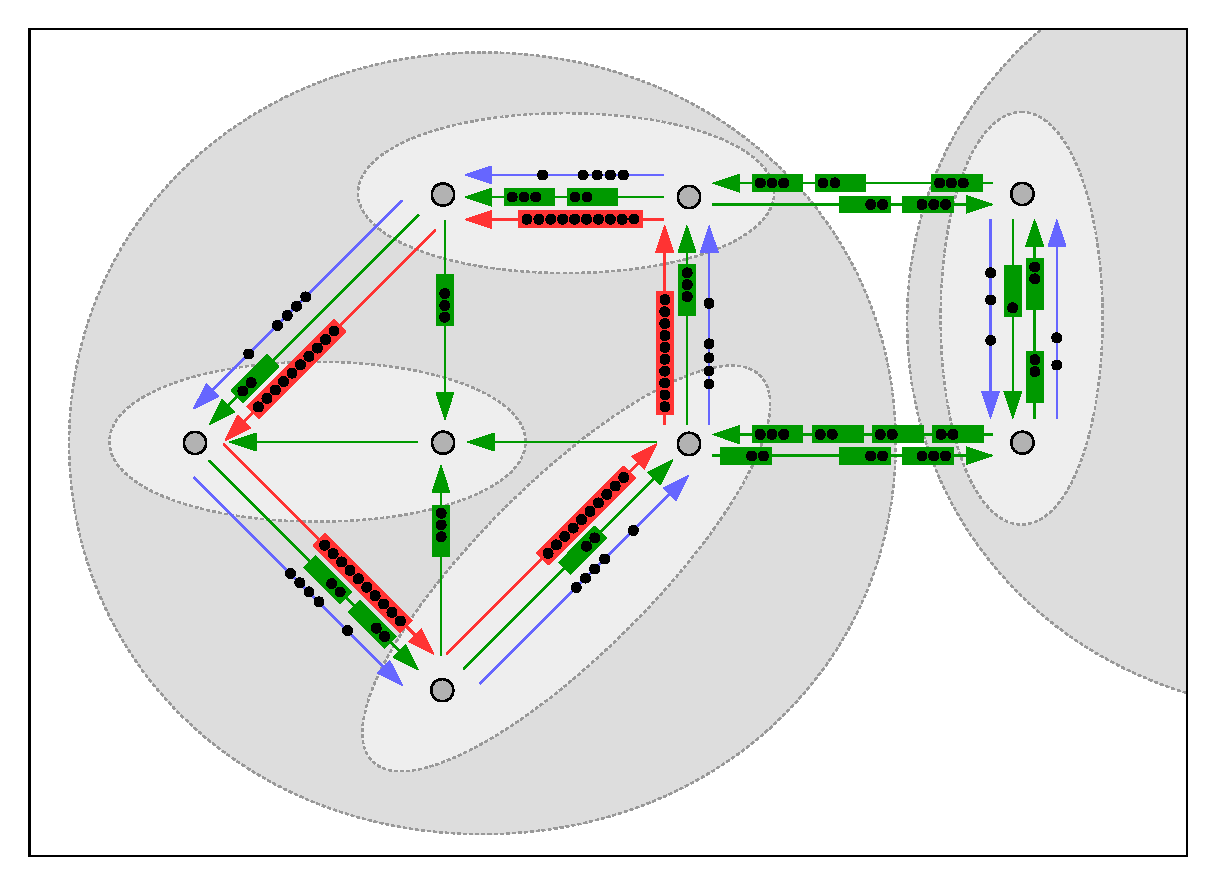
\includegraphics[width=\columnwidth]{gfx/model.pdf}
%		\caption{Illustration of integrated multi-modal passenger transport and energy flow modeling. The directed graph represents the transportation system. The nested ellipses and circles represent the power system.}
%		\label{illustration}
%	\end{figure}
	
	Section~\ref{modalities} introduces a model of transport. Section~\ref{transport} describes our model of the transport infrastructure. Section~\ref{passengers} explains our passenger model. Section~\ref{vehicles} highlights our vehicle model. Section~\ref{collisions} defines our collision criteria. Section~\ref{power} summarizes our model of the power infrastructure. Section~\ref{charging_stations} describes our model of charging stations. Section~\ref{energy_storages} explains our model of energy storages. Section~\ref{power_generators} defines our model of power generators. Finally, Section~\ref{static_loads} summarizes our model of static loads (i.e.\ non-controllable loads).
	
	\todo{How to structure this section? E.g.\ static vs.\ dynamic aspects? Transportation vs.\ power system? Contraints, objectives, ...? States, actions, ...?}
	
	\subsection{Transport infrastructures}
	\label{transport}
	Road intersections are defined by an identifier $RI$ so that
	\[
	\exists n \in \mathbb{N} : |RI| < n \mathrm{.}
	\]
	Here, intersections are made up of a given set of connectable road segments $RS$, where
	\[
	RS \subseteq RI \times RI \mathrm{.}
	\]
	
	The road segment capacity describes the number of lanes of a road segment such that
	\[
	RSL : RS \rightarrow \mathbb{N} \mathrm{,}
	\]
	while the road segment distance is defined as 
	
	\[
	RSD : RS \rightarrow \mathbb{R}^+ \mathrm{,}
	\]
	
	where road segment distance can be equal to zero when considering self-segments such that
	\[
	(ri, ri) \in RS \Rightarrow  RSD(ri, ri) = 0 \mathrm{.}
	\]
	Furthermore, road segments are defined by relative coordinates $RSC \subseteq RS \times \mathbb{R}^+ \mathrm{,}$ where, based on the segment distance
	\[
	RSC = \{(\cdot, rd) \in RS \times \mathbb{R} \mid 0 \leq rd \leq RSD(s) \} \mathrm{.}
	\]
	Then, world coordinates $WC$ describe the general geography of road segment coordinates $RSC$, defining absolute latitude, longitude as well as elevation such that
	\[
	WC : RSC \rightarrow \mathbb{R}^3 \mathrm{.}
	\]
 \todo{Do we really need that in the presentation? Can we simplify the model using world coordinates of road intersections only?}
	Finally, the traffic infrastructure $TI$ can be described as a topology such that 
	\[
	TI = (RI, RS, RSL, RSD, WC) \mathrm{.}
	\]
	
	\subsection{Passengers}
	\label{passengers}
	
	Passenger identifiers $P$ (finite set)
	\[
	\exists n \in \mathbb{N} : |P| < n
	\]
	Passenger mobility demand $PMD$ (origin position, destination position, departure time, arrival time)
	\[
		PMD \subseteq RSC \times RSC \times \mathbb{R}_0^+ \times \mathbb{R}_0^+
	\]
	Passenger state $PS$ (road segment coordinates, passenger mobility demand)
	\[
		PS : P \rightarrow RSC \times PMD
	\]
	\todo{What about passenger weight and size? Should we use those parameters? Do we need to integrate the bin-packing problem then? Is that necessary at the current stage?}
	
	\subsection{Vehicles (i.e.\ electric vehicles)}
	\label{vehicles}
	
	Vehicles $V$ (finite set)
	\[
		\exists n \in \mathbb{N} : |V| < n
	\]
	Vehicle length $VL$ (for collision detection/avoidance)
	\[
		VL : V \rightarrow \mathbb{R}^+
	\]
	Vehicle (energy) capacity $VC$ (battery size)
	\[
		VC : V \rightarrow \mathbb{R}^+
	\]
	Vehicle weight $VW$
	\[
		VW : V \rightarrow \mathbb{R}^+
	\]
	Vehicle passenger capacity $VP$
	\[
		VP : V \rightarrow \mathbb{R}^+
	\]
	Vehicle energy-efficiency $VE$ 
		\[
		VE : V \rightarrow \mathbb{R}^+
	\]
	Vehicle charge-rate $VR$ 
		\[
		VR : V \rightarrow \mathbb{R}^+
	\]
%	Vehicle goods capacity $VG$
%	\[
%		VG : V \rightarrow \mathbb{R}^+
%	\]
	Vehicle state $VS : V \rightarrow RSC \times \mathbb{R}_0^+ \times \mathbb{R}_0^+$ (road segment position, charge state) \todo{Integrate passenger assignment. Not all passengers have to be assigned. Unassigned passengers must use the pedestrian modality.}
	\[
		VS(v) \in \{ (\cdot, cs, ps) \in RSC \times \mathbb{R}_0^+ \times \mathbb{R}_0^+ \mid
	\]
	\[
		(0 \leq cs \leq VC(v)) \wedge (0 \leq ps \leq VP(v)) \}
	\]
	Vehicles states $\mathbb{VS}$ \todo{Require that passengers are not assigned multiple times! Note that we could distinguish between properties that are enforced (e.g.\ unique passenger assignment), and properties that need to be solved (e.g.\ collision-free passenger/vehicle operation).}
	\[
		\mathbb{VS} = \{VS : V \rightarrow RSC \times \mathbb{R}_0^+ \mid VS \text{ is vehicle state}\}
	\]
	\todo{Do we really need all these vehicle parameters? Maybe we can reduce the model to a few parameters only? What do we loose then?}
	
	\subsection{Collisions}
	\label{collisions}
	
	Overlapping vehicle pairs $OVP : \mathbb{VS} \rightarrow V \times V$
	\[
		OVP(VS) = \{(v_1, v_2) \in V \times V \mid
	\]
	\[
		((rs_1,rd_1),\cdot) \in VS(v_1), ((rs_2,rd_2),\cdot) \in VS(v_2) :
	\]
	\[
		rs_1 = rs_2 \wedge (|rd_1 - rd_2| < VL(v_1) / 2
	\]
	\[
		\vee
	\]
	\[
		|rd_1 - rd_2| < VL(v_2) / 2)\}
	\]
	Overlapping vehicle sets $OVS : \mathbb{VS} \times V \rightarrow \mathcal{P}(V)$
	\[
		OVS(VS,v) = \{v' \in V \mid (v, v') \in OVP(VS)\}
	\]
	Collision property $CV : \mathbb{VS} \rightarrow \mathbb{B}$
	\[
		CV(VS) \Leftrightarrow \exists v \in V :
	\]
	\[
		|OVS(VS, v)| > RSL(rs) \text{ with } ((rs,\cdot),\cdot) = VS(v)
	\]
	
	\subsection{Power infrastructures}
	\label{power}
	
	Power regions represent an aggregated representation of a set of voltage nets. For example, they can define a region based on specific low, medium or high voltage nets in a given area. However, they abstract from a detailed representation of the underlying physical net structure.  
	
	Hence, the identifier of a power region $PR$ is defined as
	\[
	\exists n \in \mathbb{N} : |PR| < n \mathrm{.}
	\]
	Power regions aggregate the loads of their subregions and connected electric devices. In return, they provide the aggregated load to their upper region.
	Hence, the acyclic parent relationship with their distinct roots $PRP$ is defined by 
	\[
	PRP : PR \to PR \mathrm{.}
	\]
	\todo{Require acyclic parent relationship with distinct root.}
	Power regions are subject to given capacity $PRC$, which describes the total load a power region can aggregate.
	The power region capacity $PRC$ is then
	\[
	PRC : PR \rightarrow \mathbb{R}^+ \mathrm{.}
	\]
	\todo{The maximum energy flow through this region.}
	 
	The current energy balance of a power region
	$PRS : PR \rightarrow \mathbb{R}_0^+$ with $cc$ describing the current capacity of an according power region is then
	\[
	PRS(pr) \in \{ cc \in \mathbb{R}_0^+ \mid 0 \leq cc \leq PRC(pr) \} \mathrm{.}
	\]
	
	\todo{Maybe we should introduce electric components here already. Then, electric components can be regions or end-points. Regions are the net identifiers introduced above. End-points are the concepts introduced in the following.}
	
	\subsection{Charging stations}
	\label{charging_stations}
	Charging stations are electric devices acting as consumers or producers within the power system. Consumption or production is based on connection to electric vehicles.
	They are defined by a identifier $CS$, where
	\[
	\exists n \in \mathbb{N} |CS| < n \mathrm{.}
	\]
	Furthermore, they have a physical coordinates on a specific road segment
	$CSP : CS \rightarrow RS$, where
	\[
	CSP(cs) = (ri_1, ri_2) \Rightarrow ri_1 = ri_2 \mathrm{.}
	\]
	\todo{Map charging station to regions.}
	
	\subsection{Energy storages}
	\label{energy_storages}
	Energy storages can store and release energy at given times.
	They are defined by an identifier $ES$, where 
	\[
	\exists n \in \mathbb{N} |ES| < n \mathrm{.}
	\]
	Here, energy storages are mapped to a specific region, e.g. determining their currently mapped voltage net.
	
	They have a fixed capacity $ESC$, which defines the total amount of energy they can store, where
	\[	
	ESC : ES \rightarrow \mathbb{R}_0^+ \mathrm{.}
	\]
	When $cc$ defines the current capacity of a energy storage, their individual state $ESS : ES \rightarrow \mathbb{R}_0^+$ is then
	
	\[
	ESS(es) \in \{cc \in \mathbb{R}_0^+ \mid 0 \leq cc \leq ESC(es)\} \mathrm{.}
	\]
	
	\todo{Use energy storages instead of power batteries (because they are more general).}
	\\
	\todo{Map power batteries to regions.}
	
	\subsection{Power generators}
	\label{power_generators}
	
	Power generators represent a class of electric devices which produce load. For example, they can represent conventional energy sources such as fossil-fuel power stations as well as renewable energy sources such as solar panels or wind turbines. For producing energy they take a resource such as coal, gas or sunlight or wind as input. Based on the input, i.e. resource employed, they produce an according output, i.e. positive load and emissions. 
	
	They are defined by an identifier $PG$, where 
	\[
	\exists n \in \mathbb{N} |PG| < n \mathrm{.}
	\]
	Power generators are mapped to specific region, e.g. determining their currently mapped voltage net.
	Concerning environmental factors, power generator emissions $PGE$ define the total emissions which occur during power production in a time instant.
	\[
	PGP : PG \rightarrow \mathbb{R}_0^+ \mathrm{.}
	\]
	
	Power production is based on their individual power efficiency $SPS$, which defines the total amount of energy they can produce as an output, given a specific resource they utilize.
	\[	
	PGP : PG \rightarrow \mathbb{R}_0^+ \mathrm{.}
	\]
%	
%	Solar panel identifiers $SP$
%	\[
%		\exists n \in \mathbb{N} : |SP| < n
%	\]
%	Solar panel power scale $SPS$ 
%	\[
%		SPS : SP \rightarrow \mathbb{R}^+
%	\]
%	Solar panel power $SPP$ 
%	\[
%		SPP : SP \times \mathbb{R}^+ \rightarrow \mathbb{R}^+
%	\]
%	
	
	\todo{Use power generators instead of solar panels (because they are more general). Then we have to model the emissions (CO2, noise, etc.) also! Solar panels do not cause any emissions (only during production and maintenance).}
	\\
	\todo{Map power generators to regions.}
	
	\subsection{Static (i.e.\ non-controllable) loads}
	\label{static_loads}
	\todo{Represent non-controllable energy production and consumption. For example, activities such as cooking or watching television are non-controllable in our model. In general, the loads can be selected according to the use case.}
	Static loads represent an aggregation of devices within the power system with non-controllable loads, i.e. energy production or consumption. 
	They are defined by an identifier $SL$, where 
	\[
	\exists n \in \mathbb{N} |SL| < n \mathrm{.}
	\]
		
	They abstract from details regarding specific behavior of specific electric devices.
	For example, static loads can represent an aggregation of activities with non-controllable loads with human interaction such as cooking or watching television. Based on their selected profile for the given use case, static loads exert different behavior.
	Hence, a given static load profile $SLP$ describes the according load per time instant only, where
	\[
	SLP : SL \times \mathbb{R}_0^+ \rightarrow \mathbb{R} \times \mathbb{R} \mathrm{.}
	\]
	Here, static loads are mapped to a specific region, e.g. determining their currently mapped voltage net.
	\todo{Map static loads to regions.}
	
	\subsection{Contraints}
	
	\todo{What are the constraints in our model? Vehicle collision, vehicle overloading, electric net capacity overloading, ...}
	
	\subsection{Objectives}
	
	\todo{What are the objectives in our model? Derivation from departure time, derivation from arrival time, derivation from departure road segment, derivation from arrival road segment, emissions, ...}
	
	\section{Case Study}
	
	\todo{Previous results shown in ICCVE-2015.}
	
	\section{Discussion}
	\label{discussion}
	
	\todo{Write discussion. What does the model capture? How well does the model capture this information? What does the model not capture? When do we need the information that is not captured? When don't we need the information that is not captured?}
	
	\section{Conclusion}
	\label{conclusion}
	
	\todo{Write conclusion. How far are we in modeling the problem? When can we use the model for real-world scenarios? How far are we in solving the problem?}
	
	\bibliographystyle{bst/IEEEtran}
	\bibliography{references}
	
\end{document}